\chapter{Experimental}

%\emph{\color{gray}Probably need to mention CCD digitaztion pedestal and noise, and dark counts which are zero when cold -- did you do that?.}

%\noindent
%\emph{

This chapter describes the apparatus at Colorado State University that was used for producing and observing  deposits of Ba and Ba\textsuperscript{+} in SXe.  The main barium source, a Ba\textsuperscript{+} ion beam, is first described in Sec. \ref{sec:ionbeam}, and then a neutral Ba getter source is discussed in Sec. \ref{sec:getter}.  The co-deposit of Ba or Ba\textsuperscript{+} with Xe gas onto a cold sapphire window is described in Sec. \ref{sec:deposition}.  The technique for focusing the laser into the SXe is described in Sec. \ref{sec:laser}, and imaging of the laser region is described in Sec. \ref{sec:collection}, with attention to the effect of vibrations in Sec. \ref{sec:vibes}.  Finally, a system for scanning the focused laser across the sapphire window is described in Sec. \ref{sec:laserscanning}.

\section{Ion Beam}
\label{sec:ionbeam}

The Colutron ion beam system is a clean mass-selected source of Ba\textsuperscript{+} which, with the added capability of pulsing, can do a very wide range of deposit sizes, from billions of ions in a focused laser region all the way down to the single-ion level and below.  The different components of this system are shown in Fig. \ref{fig:ionbeam} and described in the following subsections.  Ions produced in a Colutron ion source receptacle are accelerated and collimated for passage through the mass filter.  Several sets of deflection plates are available for steering, and Einzel lenses focus the beam near the final Faraday cup.  A set of pulsing plates can be used to deposit 1-$\mu$s, or continuous ion current can be used in depositing in SXe on the cold sapphire window.
%(may only want to say that if we have those scans)

\vspace{20mm}

%\begin{landscape}
\begin{figure} %[H]
        \centering
                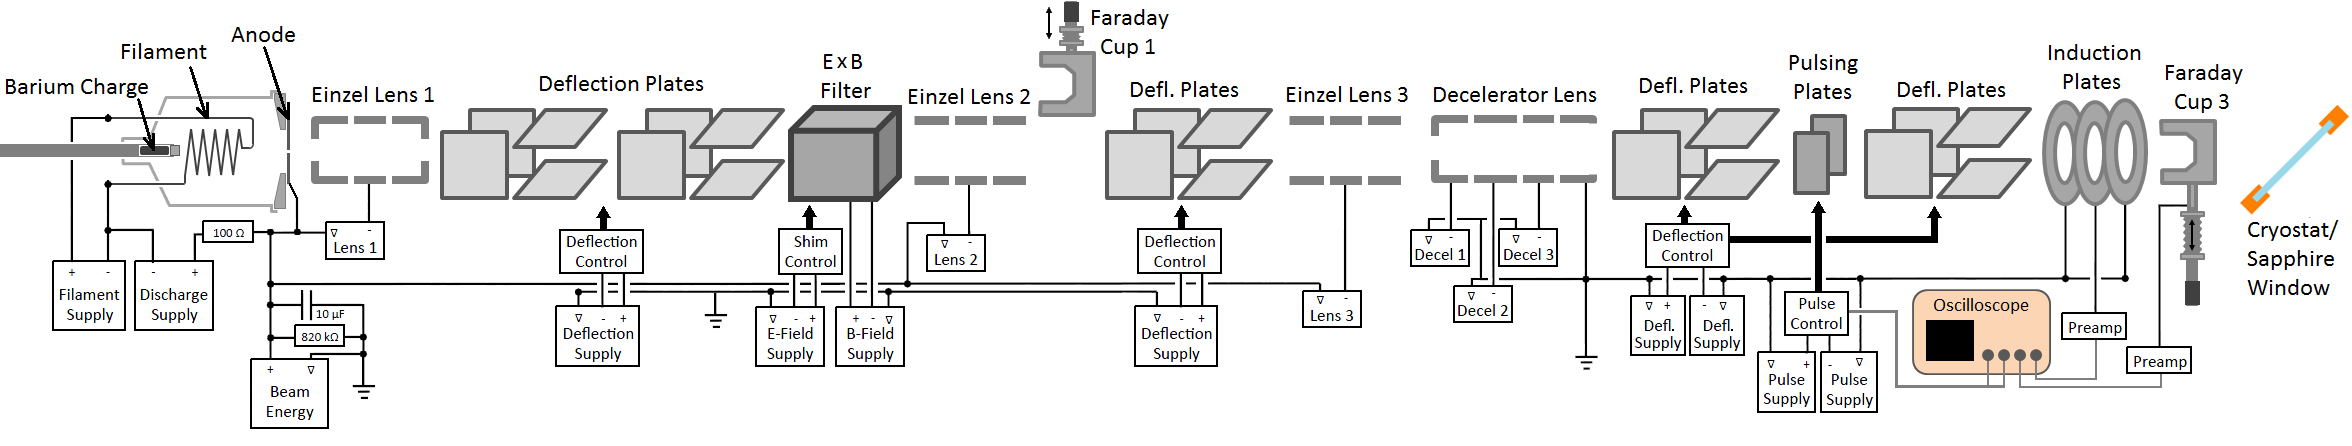
\includegraphics[angle=90,width=.25\textwidth]{figures/ionBeam.png} %angle=90,
                \caption{Ba\textsuperscript{+} ion beam.}
\label{fig:ionbeam}
\end{figure}
%\end{landscape}
%width=1.4 is good for landscape, but idk how to get it in the center

\subsection{Ion Source}

Ba\textsuperscript{+} ions are produced in the source of a Model DCIS-101 Colutron ion gun \cite{Colutron}.  It is shown in Fig. \ref{fig:ionsource}.  A solid Ba charge is placed into the hollowed end of a stainless steel rod, which is capped by a loose screw.  The source rod is inserted into the discharge chamber, where it is heated by a filament, vaporizing the Ba.  The source is designed to produce a discharge between the anode plate and the filament cathode, through an argon buffer gas leaked into the source chamber.  This controlled discharge also ionizes Ba atoms from the solid charge to produce the desired Ba\textsuperscript{+} ion beam, and the Ar\textsuperscript{+} ions are filtered out.  In the present work, to avoid contamination of the SXe matrix with residual Ar gas, the buffer gas was not used.  It has been found that, with care, the discharge can be maintained with Ba vapor alone.  The longevity of ion current from a single charge is at least several 10s of hours.  This suggests that Ba is coating the inner walls of the source chamber, and is heated enough to provide sufficient Ba pressure to support a discharge.

The discharge produces a plasma, containing barium ions.  The application of an acceleration potential draws Ba\textsuperscript{+} ions from the plasma.  The 2~kV acceleration potential is applied between the ion source anode and the first element of Einzel lens 1 (L1).  The potential of this lens is adjusted to collimate the ion beam for passage through the E$\times$B velocity filter.

%This is supported by the observation of white oxidation of the inner source parts after a few minutes of exposure to air when opening the system.

\begin{figure} %[H]
        \centering
                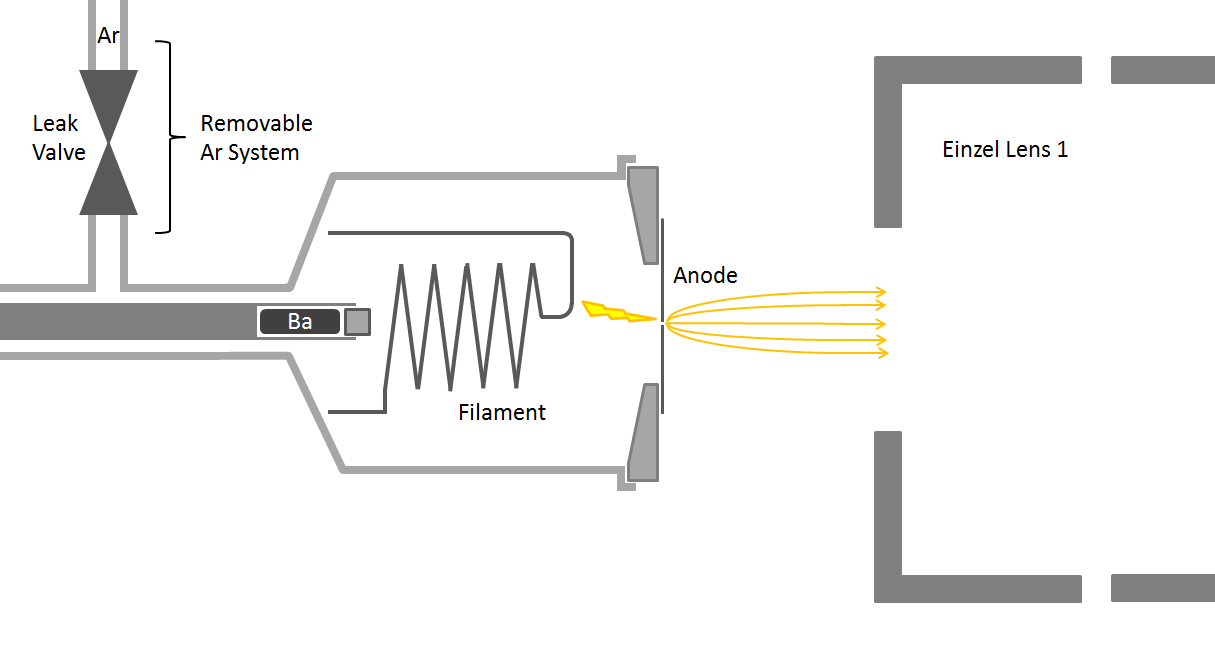
\includegraphics[width=.95\textwidth]{figures/ionSource.png}
                \caption{Ba\textsuperscript{+}/Ar\textsuperscript{+} ion source.}
\label{fig:ionsource}
\end{figure}

\subsection{E$\times$B Velocity Filter}

The E$\times$B velocity filter selects Ba\textsuperscript{+} by creating perpendicular electric and magnetic fields, which produce opposing forces on charged particles moving through the filter.  The opposing forces will be equal for ions with velocity $v = \frac{E}{B}$.  Since ion velocity is determined by mass ($m$), charge ($q$) and beam potential ($V$), the filter selects ions satisfying Eq. \ref{eqn:massfilt}:

\begin{equation}
\frac{m}{q} = \frac{2 V B^{2}}{E^{2}}
\label{eqn:massfilt}
\end{equation}

\noindent
where $B$ and $E$ are the magnetic and electric fields, respectively.  Those fields are chosen such that Ba\textsuperscript{+} ions pass straight through.  Other ions will be deflected.  

The E$\times$B filter is shown in Fig. \ref{fig:exb}.  Electromagnets provide a vertical magnetic field.  Electrode plates and field-shaping guard rings provide a horizontal electric field.  The guard rings prevent lensing and astigmatism from fringe fields of the plates \cite{Colutron}.

\begin{figure}[h]
        \centering
                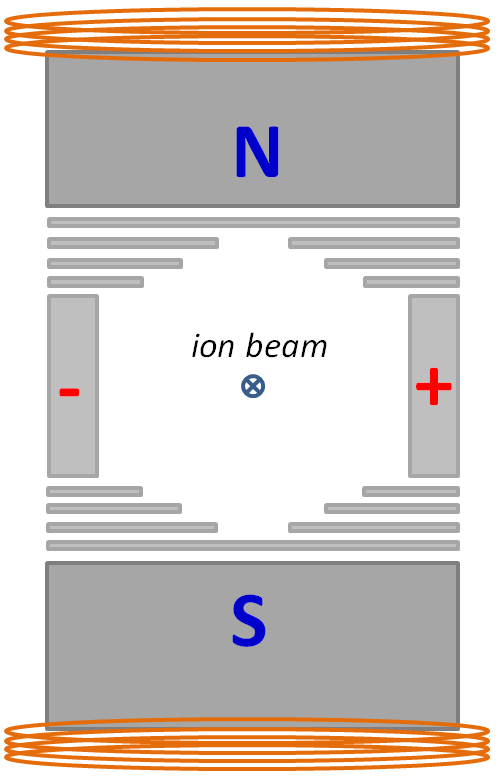
\includegraphics[width=.7\textwidth]{figures/ExB.png}
                \caption{Colutron E$\times$B ion velocity filter.}
\label{fig:exb}
\end{figure}

%\emph{\color{gray}If we need mass scans, we probably need to do new ones with a constant magnetic field, and Ar\textsuperscript{+} and Ba\textsuperscript{+} in same day.  Past scans were all over the place, partly because we were changing beam settings, but new peaks are not very consistent either.}
%To determine the mass components of the beam, the electric field can be scanned.  Mass scans of the Ba\textsuperscript{+} beam is shown in Fig. [ref mass scan fig], as well as of an Ar\textsuperscript{+} beam.  The known mass of Ar aids in calibrating the magnetic field, which differs from the calculation given by Colutron, likely due to hysteresis in the magnet.  \emph{\color{gray}The Ba\textsuperscript{+} peak agrees with the Ba mas s... }

\subsection{Other Beam Components}

The first three sets of deflection plates shown in Fig. \ref{fig:ionbeam} can be used for beam diagnostics, and are set to 0~V during normal operation.  The fourth set of deflection plates, H1 and V1, located just before the pulsing plates are set to constant values of +50~V and 0~V, respectively.  These voltages have been selected such that the beam, in both pulsing and continuous modes, can be deposited at the sapphire window for reasonable settings on the final deflection plates, H2 and V2.  As described in Section \ref{subsec:ionDepCal}, different settings in H2/V2 are required for peak ion current in Faraday cup 3 vs. peak deposit at the window.

Einzel lens 2 (L2) focuses the beam to pass through the aperture in the first element of the decelerator lens.  Einzel lens 3 (L3) is set to zero in this setup.  The decelerator lens can be used to vary Ba\textsuperscript{+} deposit energy, which was done in \cite{Shon}, but in this work it acts as an Einzel lens with only the second element (D2) at non-zero voltage.  It focuses the beam near the sample and Faraday cup 3 (there is no Faraday cup 2 in this setup).

Faraday cup 3 measures the ion current during experiments, and is retracted when deposits are being made.  Calibration of deposits using Faraday cup 3 is described in Section \ref{subsec:ionDepCal}.  Faraday cup 1 can be used for beam diagnostics, and is usually retracted.  An additional Faraday cup, cup W, can be attached to the coldfinger in place of the sapphire window for determining deflection plate voltages for depositing Ba\textsuperscript{+} on the sapphire window, and for calibrating ion deposits.  This is described further in Sec. \ref{subsec:ionDepCal}.

To align the ion beam, L1 was first tuned to maximize ion current in Faraday cup 3, with L2, L3, and D2 set to zero.  Since cup 3 is about 2~m away from L1, this approximately collimates the beam for passage through the E$\times$B filter.  The optimal value for L1 was found to be around -400~V relative to the 2000~V beam energy.  Next, L2 and D2 were fine-tuned together to achieve maximal current in cup 3.  Finally, the straightness of the beam was checked by peaking ion current with deflection plates H1 and V1 on cup 3 and cup W.

%\emph{\color{red}consistent with Bill's SIMION -- show?}

%L2 8.34 = 

\subsection{Ion Beam Pulsing}

To deposit small numbers of ions, it is desirable to be able to pulse the ion beam with short pulses.  To achieve pulsed beams, the pulsing plates, normally set to 200~V and -200~V to deflect the beam, are pulsed to 0~V for 1~$\mu$s to pass a short pulse of ions straight forward.  The pulsing circuit is shown in Fig. \ref{fig:pulse_circuit}.  Square waves, triggered by LabVIEW at 500~Hz, enter the circuit at (a). A transformer isolates a MOSFET switch from ground.  Upon a trigger pulse the MOSFET switch shorts the pulsing plates for the period of the pulse.

\begin{figure} %[h]
        \centering
                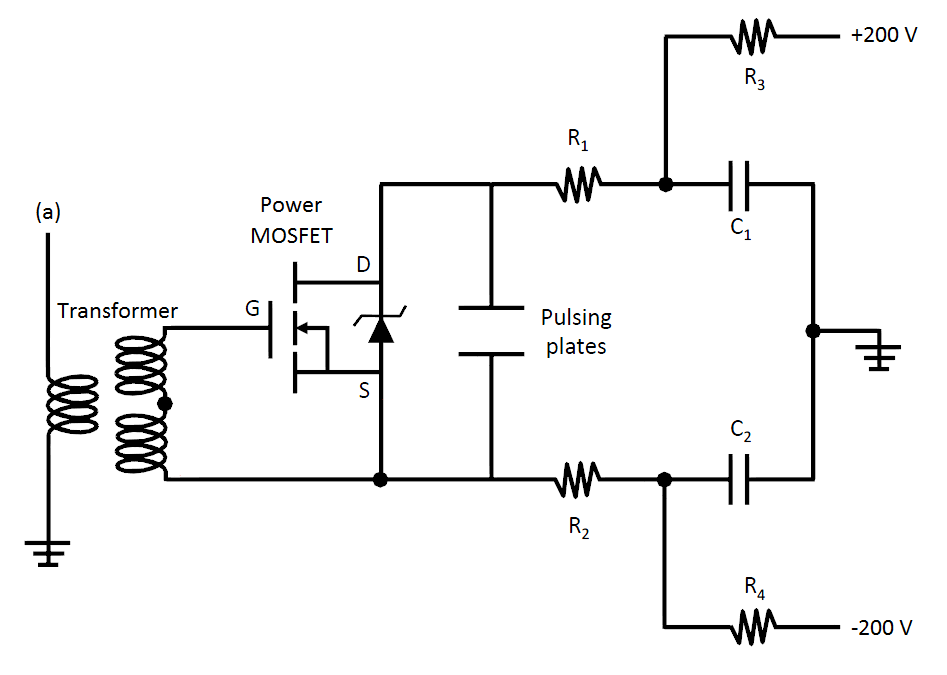
\includegraphics[width=.85\textwidth]{figures/pulsing_circuit.png}
                \caption{Pulsing circuit.  R$_{1}$ = R$_{2}$ = $470~\Omega$, R$_{3}$ = R$_{4}$ = 20~k$\Omega$, \newline C$_{1}$ = C$_{2}$ = 680~nF. \cite{Shon}}
\label{fig:pulse_circuit}
\end{figure}

The pulsing plates are followed by three induction plates, the middle plate of which provides a measure of the ion pulses.  Just prior to a deposit, the charge in the pulses can be directly measured on cup 3.  eV Products pre-amplifiers convert the ion current in the induction plates and cup 3 (or cup W) to voltage signals, which are recorded on a digital oscilloscope.  An example of raw oscilloscope traces of Faraday cup 3 and induction plate signals are shown in Fig. \ref{fig:pulse_raw_shaped}(a).  The pre-amp output voltage is related to the input current according to Eq. \ref{eqn:preamp}:

\begin{equation}
I = \frac{-(V_{out} + R_{1} C \frac{dV_{out}}{dt})}{R_{1} M}
\label{eqn:preamp}
\end{equation}

\noindent
where $R_{1} C$ and $R_{1} M$ are determined by putting a known square pulse of current into the pre-amp through a large resistor.  First, the time constant of an exponential fit to the signal decay after the pulse determines $R_{1} C$.  Then $R_{1} M$ is determined by matching this shaped signal to the original square pulse.  The actual currents in the induction plates and cup 3 derived using Eq. \ref{eqn:preamp} are shown in Fig. \ref{fig:pulse_raw_shaped}(b).  The induction signal is positive as ions are approaching the middle plate, and an equal but negative signal is seen after the ions pass through.  The Faraday cup stops the ions, so it produces only a positive induction signal as ions approach it.

\begin{figure} %[H]
        %\centering
        %\begin{subfigure}
                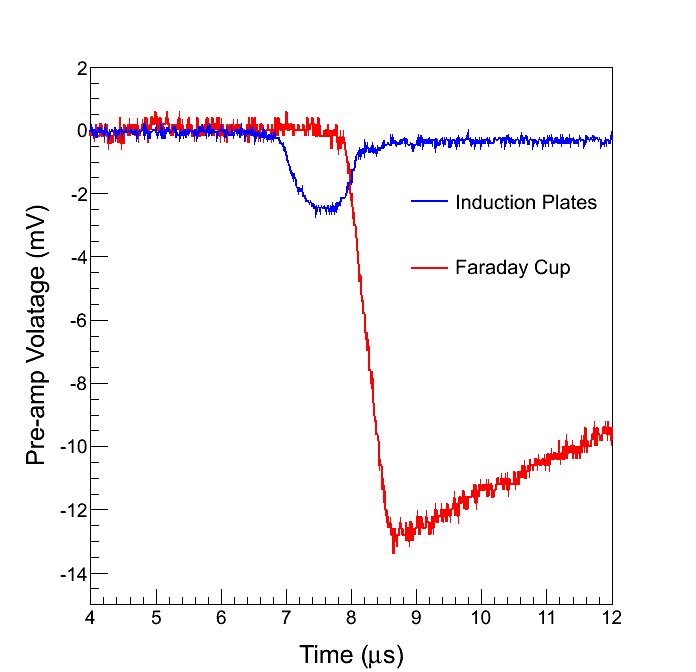
\includegraphics[width=.49\textwidth]{figures/pulse_ind_cup3_raw.png}
                %\caption{barf}
%        %\end{subfigure}
        %\begin{subfigure}
                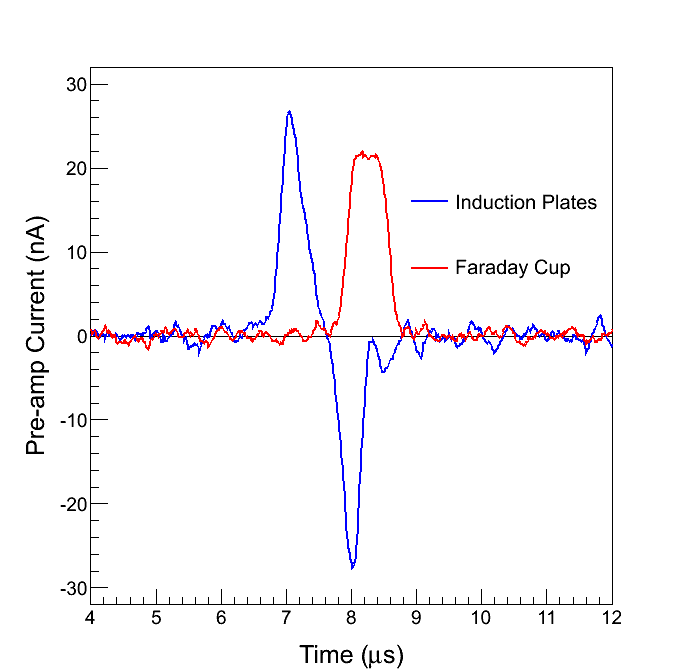
\includegraphics[width=.49\textwidth]{figures/pulse_ind_cup3_shaped.png}
                \caption{Raw (a) and shaped (b) pulse signals from induction plates and cup 3.  The raw induction signal appears small because it is a less sensitive pre-amp (accounted for in shaping).}
        %\end{subfigure}
        \label{fig:pulse_raw_shaped}
\end{figure}

Pulsing data also provide confirmation that the beam is composed of Ba\textsuperscript{+}.  The time between the center of the pulsing plate voltage overlap and the center of the pulse measured by the Faraday cup, along with the known distance traveled, determines the velocity measurement of the ions.  The distance from the center of the pulsing plates to the Faraday cup was measured to be 31.5 $\pm$ 0.5~cm.  Time-of-flight data, e.g. Fig. \ref{fig:pulses_ArBa}, give 39.8 $\pm$ 3.4~amu for Ar\textsuperscript{+} ions and 136.8 $\pm$ 6.3~amu for Ba\textsuperscript{+} ions, including an uncertainty on the time of flight of $\pm$ 0.1~$\mu s$.  These agree with the known atomic masses.

\begin{figure}[h]
        \centering
                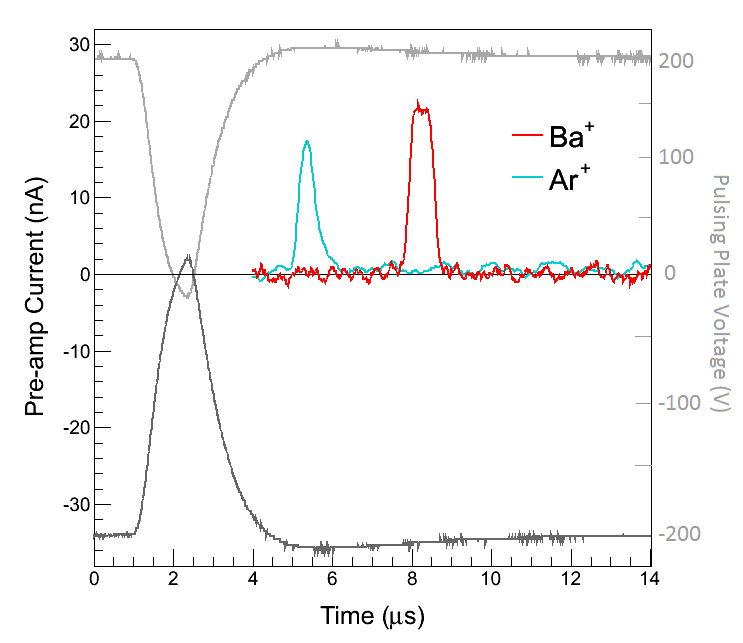
\includegraphics[width=.7\textwidth]{figures/pulses_BaAr.png}
                \caption{Arrival time of pulses at cup 3 vs. time of pulsing plate signal (black (+) and gray (-)) for Ar\textsuperscript{+} and Ba\textsuperscript{+} ions at 2000~eV.}
\label{fig:pulses_ArBa}
\end{figure}

\subsection{Calibration of Ion Deposits}
\label{subsec:ionDepCal}

The ratio of between ion current in cup 3 and cup W is measured to be $0.5 \equiv r_{\text{w}}$.  Then, the ion density per pulse at the sapphire window is defined by:

\begin{equation}
\frac{\text{ions}}{\text{pulse} \times m^{2}} = \frac{Q r_{\text{w}}}{e A}
\label{eqn:ion_density}
\end{equation}

\noindent
where $Q$ is the charge/pulse at cup 3, $A$ is the area of cup W, and $e$ is the elementary charge.  The radius of the opening in cup W is 1.4~mm.  Each time cup W is inserted, the voltages on the final deflection plates H2 and V2 which optimize the signal in cup W, in pulsed and continuous mode, are determined.  In the latest imaging experiments, these differed from the values for maximum cup 3 signal by about 70~V in H2 and 60~V in V2, corresponding to an effect of the undeflected beam of about 4~mm in x and y position at cup W relative to the center line from cup 3.  This indicates the level of drift in optimal ion beam component settings that occur over time.

\section{Ba Getter Source}
\label{sec:getter}

A BaAl$_{4}$ getter, manufactured by SAES with part number ST 2/F/WIRE, can be inserted on a bellows to emit toward the sapphire window, as shown in Fig. \ref{fig:endOfBeamBa}.  When heated, the getter emits neutral Ba with minimal Ba\textsuperscript{+} due to the low temperature ($\sim$800$^{\circ}$ C determined by observing brick red color temperature).  Getters were used extensively in previous work \cite{Brian} for measuring the absorption and emission spectra of Ba in SXe with large Ba deposits.  A getter was used briefly in this work in verifying that the 619-nm fluorescence peak, that is used for single Ba imaging, is actually a neutral Ba peak, as described in Section \ref{sec:619identification}.  The barium getters used in \cite{Brian} were exothermic BaAl$_{4}$-Ni flash getters.  The getter used here is an endothermic BaAl$_{4}$ type, designed for more controlled Ba emission.  

%no evidence is provided in Brian's thesis, nor Shon's, and I don't see anything on the SAES website

\begin{figure} %[h]
        \centering
                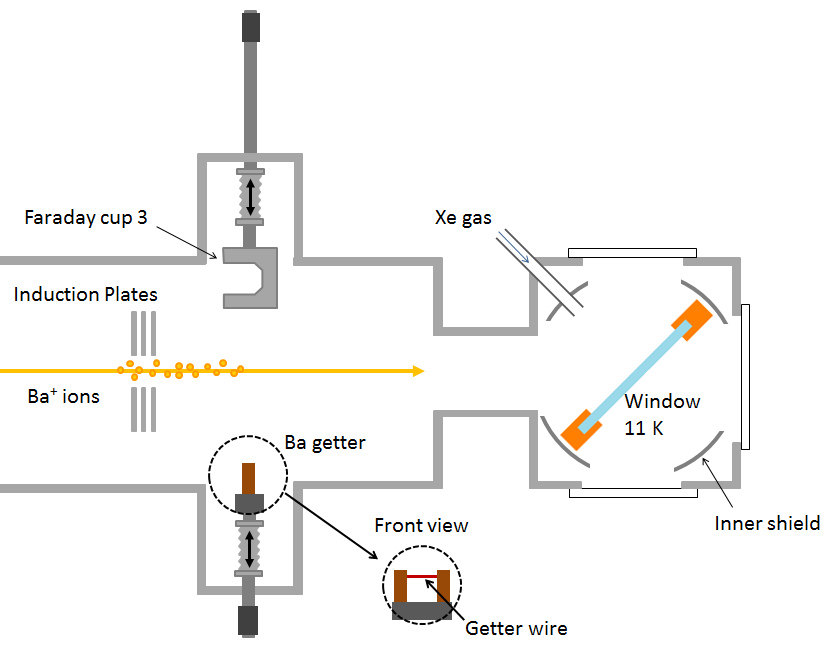
\includegraphics[width=.75\textwidth]{figures/window_etc_justBa_frontViewGetter.png}
                \caption{Apparatus near sapphire window, including induction plates, Ba getter, Faraday cup 3, Xe gas inlet, and sapphire window at 11~K.}
\label{fig:endOfBeamBa}
\end{figure}

%\begin{figure} %[h]
%        \centering
%                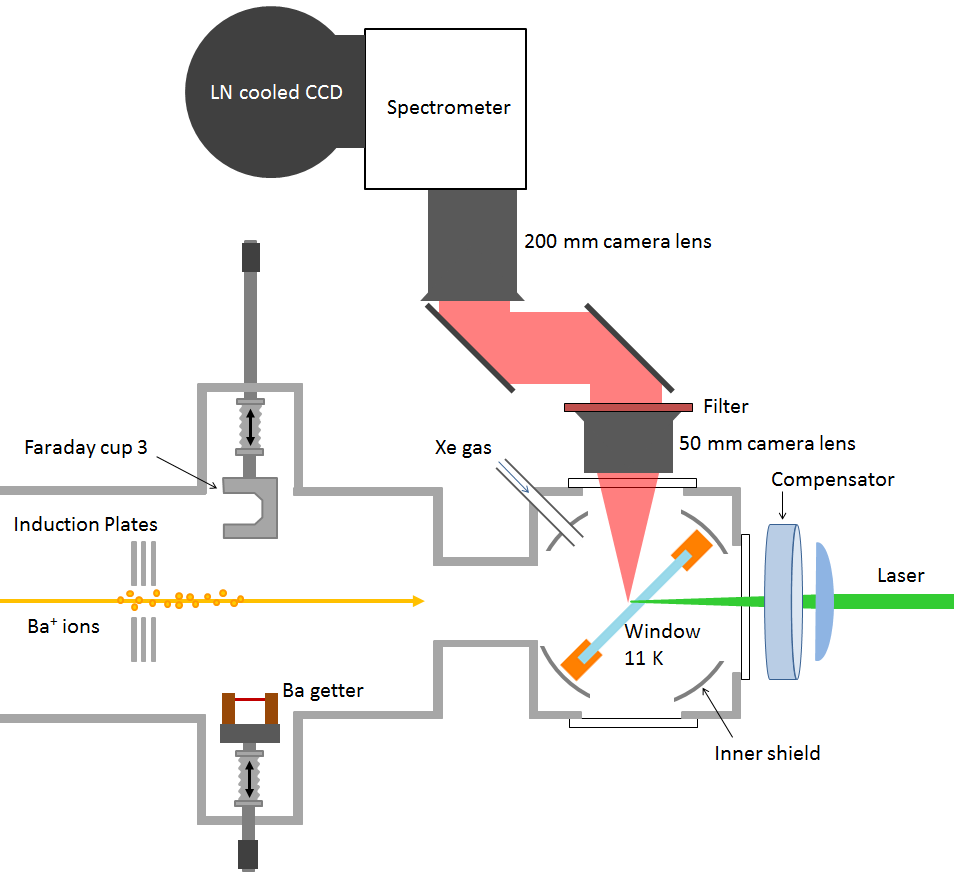
\includegraphics[width=.9\textwidth]{figures/window_etc.png}
%                \caption{Apparatus in spectroscopy region, including Ba getter, Faraday cup 3, induction plates, and optics for excitation, fluorescence collection, spectroscopy and detection.}
%\label{fig:endOfBeam}
%\end{figure}

\section{Sample Deposition}
\label{sec:deposition}

The Ba\textsuperscript{+}/Ba is co-deposited with 99.995\% purity Xe gas onto a cold sapphire window.  Sapphire has good thermal conductivity at low temperature and good optical transparency in the visible.  The window is held in a copper mount attached to a coldfinger and is tilted at 45$^{\circ}$ to allow access of the ion beam and Xe gas, as well as the excitation laser and collection optics.  To begin a deposit, Xe gas is flowed toward the window via a leak valve, through an inlet system designed and built by Brian Mong and Shon Cook \cite{Brian,Shon}.  Cup 3 is then retracted and the pulsing plates are pulsed to zero volts, depositing 1-$\mu$s pulses of Ba\textsuperscript{+} ions into the SXe matrix as it grows.  Cup 3 is then replaced, and the Xe leak stopped.

\begin{figure} %[h]
        \centering
                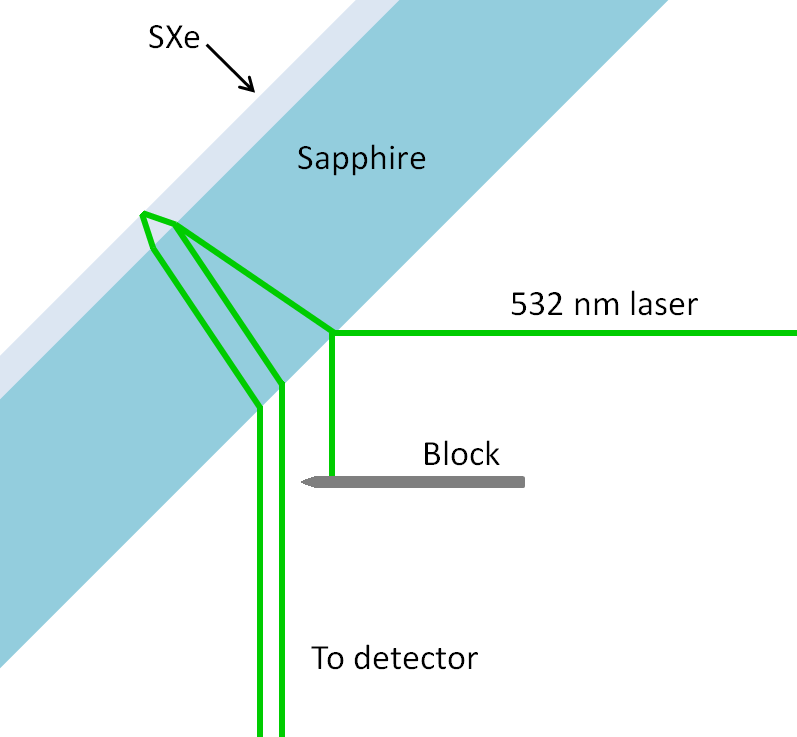
\includegraphics[width=.4\textwidth]{figures/fringe_setup.png}
                \caption{Setup for measuring SXe deposition rate by interference fringes.}
\label{fig:fringe_setup}
\end{figure}

\begin{figure} %[h]
        \centering
                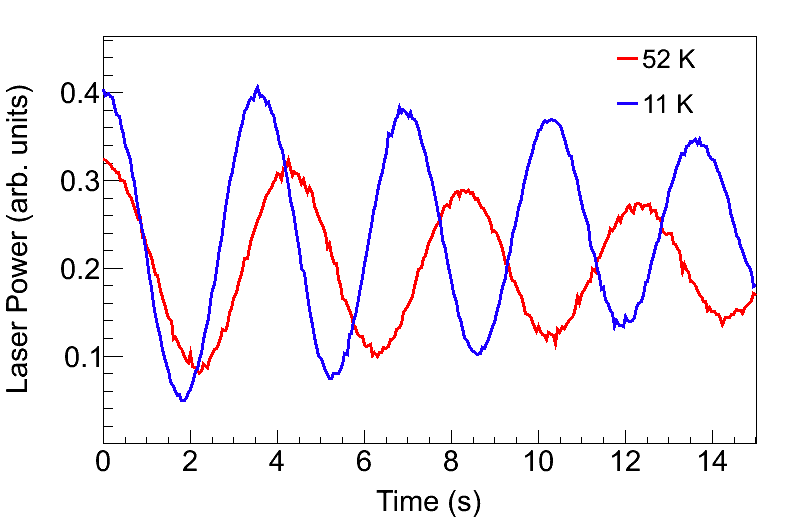
\includegraphics[width=.5\textwidth]{figures/fringes_52K_vs_11K.png}
                ~
                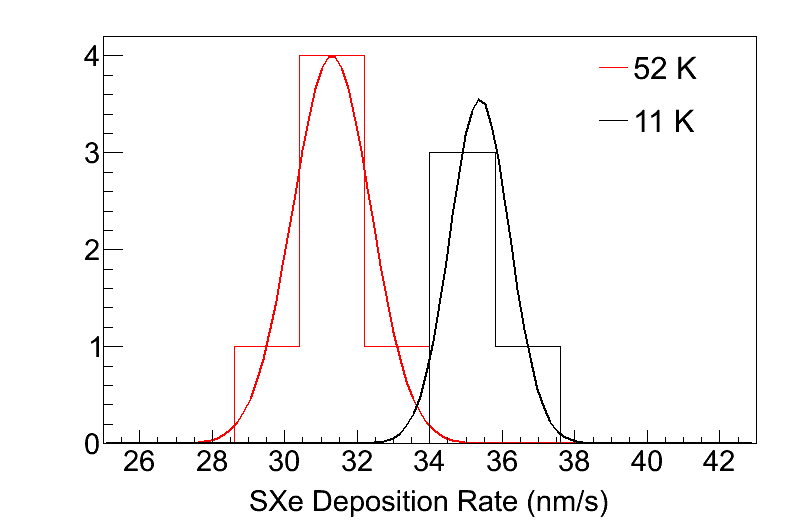
\includegraphics[width=.5\textwidth]{figures/fringes_52K_vs_11K_statistics.png}
                \caption{(a) Interference fringes for the same Xe gas leak rate deposited on the sapphire window at 11~K and at 52~K, and (b) distribution of SXe deposition rates calculated from fringe period of several measurements.}
\label{fig:fringes_52K_vs_11K}
\end{figure}

The SXe matrix deposition rates have been measured by interference fringes in a laser reflected from the front surface of the sapphire window and the SXe surface, as shown in Fig. \ref{fig:fringe_setup}.  Fringes for SXe deposition at 52~K and 11~K are shown in Fig. \ref{fig:fringes_52K_vs_11K}(a) for the typical leak rate used in this work.  The refractive index of SXe has a negligible dependence on temperature between 50~ and 30~K \cite{SXeIndex}, so these rates can be compared directly.  A distribution of SXe deposition rate measurements from several deposits is shown in Fig. \ref{fig:fringes_52K_vs_11K}(b).  A rate of $31.2 \pm 0.9$~nm/s is measured for deposits at 52~K, and a somewhat higher rate of $35.6 \pm 0.9$~nm/s is measured for deposits at 11~K.

%A somewhat lower rate is observed at 52~K, $31.3 \pm 0.44(\text{stat}) \pm 0.31(\text{sys})$~nm/s, vs. $35.4 \pm 0.41(\text{stat}) \pm 0.35(\text{sys})$~nm/s at 11~K.  Statistical errors are $\sigma / \sqrt{N}$ where $\sigma$ is the standard deviation of the Gaussian fits to the distributions in Fig. \ref{fig:fringes_52K_vs_11K}(b), and $N$ is the number of entries.  Systematic errors come from propagating an uncertainty on the angle between the laser and sapphire window of $\pm 2^{\circ}$.

\begin{figure} %[h]
        \centering
                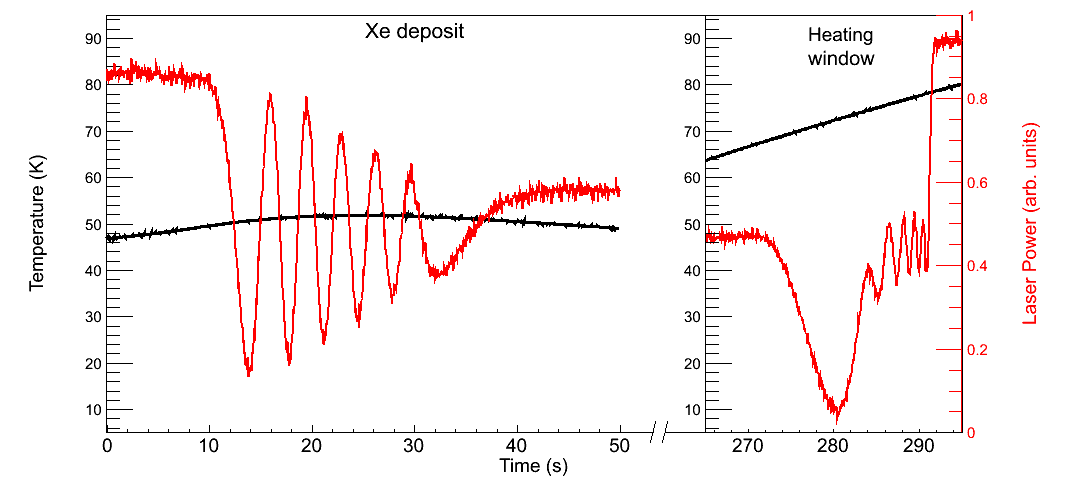
\includegraphics[width=.9\textwidth]{figures/fringes_dep_and_melt.png}
                \caption{Interference fringes of a deposit at 52~K and of its subsequent evaporation when heating the sapphire window, and temperature vs. time curves.}
\label{fig:fringes_melt_withDep}
\end{figure}

To evaporate a sample, the window is heated to 100~K.  Fringes appear during this process as well.  The full set of fringes for a deposit at 52~K and its evaporation when heated is shown in Fig. \ref{fig:fringes_melt_withDep}, along with the window temperature.  It is observed that the SXe evaporates between 73~K and 78~K.  The same number of fringes appear in the deposit and the evaporation, indicating that the lower deposition rate at around 50~K is not due to simultaneous evaporation, but perhaps due to a different sticking coefficient.  The variance in temperature during the deposit is due to the heater cycle.  These Xe deposits were for a longer time than in a typical deposit during a fluorescence experiment, in order to observe several fringes.

%quadrature errors: 0.54 for 52 K and 

%where sh'ew put this? sh'we?  these numbers are apparently wrong anyway   {\color{red}Using the 10~K SXe density of 3.780~g/cm\textsuperscript{3} \cite{SXeDensity} and a typical Ba\textsuperscript{+} ion current density of 1.6~nA/mm\textsuperscript{2} at the sapphire window, \emph{\color{gray}Re-do this, ala procedure in thought\_process.pptx, since you don't claim 37 nm/s anymore:} 5~nm/s \emph{\color{gray}any other instances?} and 37~nm/s correspond to Xe:Ba ratios of about $8.7 \times 10^{3}$ and $6.4 \times 10^{4}$ respectively.  Xe leak rates above 37~nm/s result in rapid frosting of the SXe matrix, which causes blurring of the image and high laser scatter.}

\section{Laser Excitation}
\label{sec:laser}

\begin{figure} %[h]
        \centering
                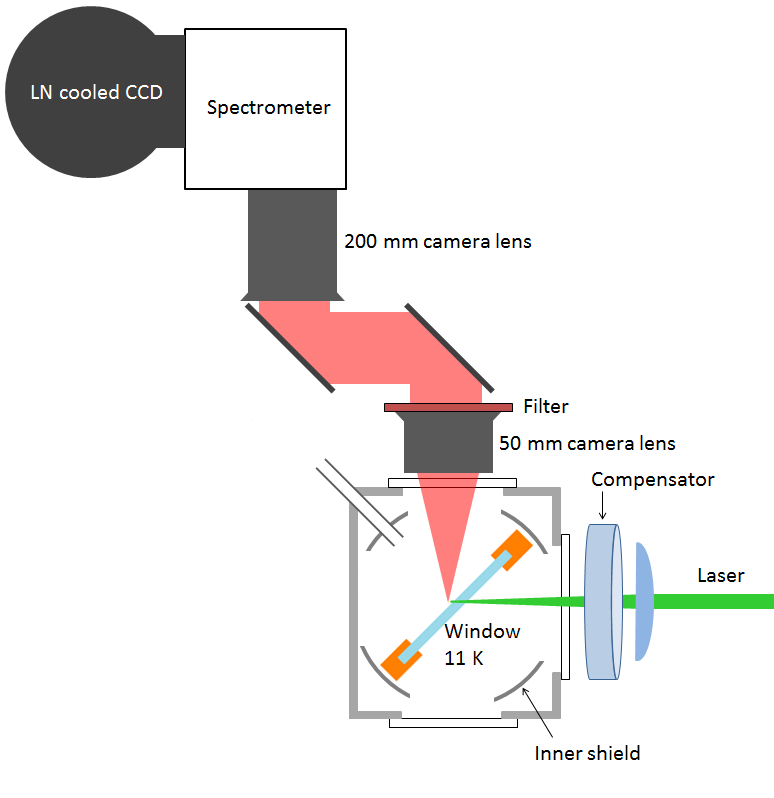
\includegraphics[width=.7\textwidth]{figures/window_etc_justOptics.png}
                \caption{Apparatus in spectroscopy region, including optics for excitation, fluorescence collection, spectroscopy and detection.}
\label{fig:endOfBeamOptics}
\end{figure}

Green to yellow laser excitation is done with a Coherent 599 dye laser, pumped by the 514-nm line of a Lexel 3500 Ar ion laser.  Rhodamine 110 (R110) dye is used for the 542 - 566~nm wavelength range, and Rhodamine 6G (R6G) for the 567 - 590~nm range.  Another Coherent 599 dye laser with Coumarin 480 (C480) dye is used for blue excitation, which is pumped by a Kr ion laser.  The Coherent 599 dye lasers are used with birefringent filters for wavelength tuning, but without etalons or single frequency stabilization, since the broad absorption of Ba in SXe does not require narrow band laser excitation.

\begin{figure} %[h]
        \centering
                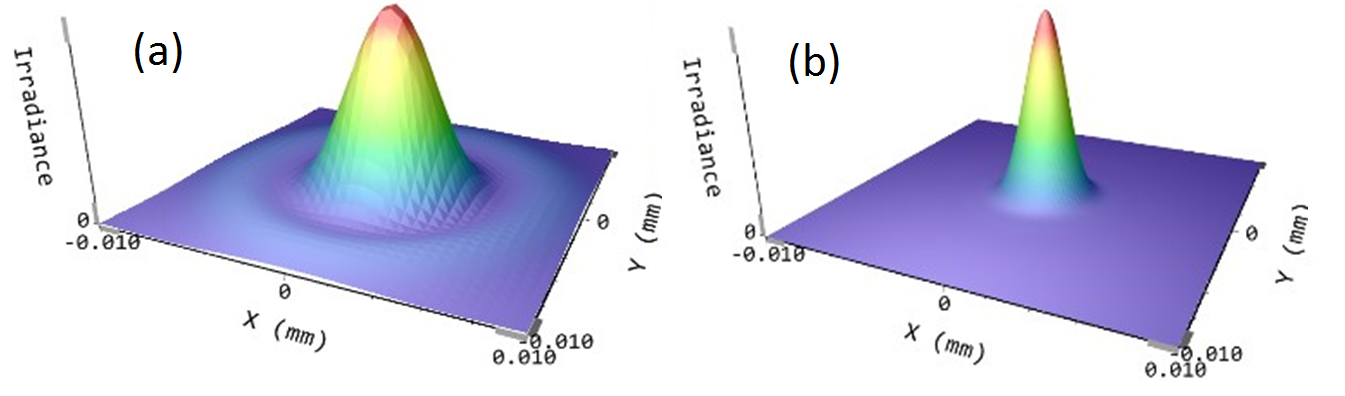
\includegraphics[width=.7\textwidth]{figures/DFairbank_aber.png}
                \caption{Calculated minimum laser spot size distributions, with wavelength 570~nm and incident laser radius w = 7~mm, for (a) bi-convex f = 7~cm lens, and (b) aspherical f = 7.9~cm lens.  \cite{DFairbank}}
\label{fig:DFairbank}
\end{figure}

The optics for these experiments is shown in Fig. \ref{fig:endOfBeamOptics}.  In initial work, including spectroscopy (Chapter \ref{chapter:spectroscopy}) and some imaging (Chapter \ref{chapter:imaging}), a bi-convex was used.  This lens had a little spherical aberration, resulting in blurring of the laser focus.  This aberration does not affect the spectroscopy results in Chapter \ref{chapter:spectroscopy}, where semi-focused beam 1/$e^{2}$ radii of 100-1000~$\mu$m were used.  However, spherical aberrations caused the minimum beam radius to be about 5~$mu$m.  To approach the diffraction limit in imaging small numbers (Chapter \ref{chapter:imaging}), a 7.9-cm focal length aspherical lens was used.  A comparison of the minimum spot sizes for these two lenses, calculated by David Fairbank with Thorlabs software, is shown in Fig. \ref{fig:DFairbank}.

\begin{figure} %[H]
        \centering
                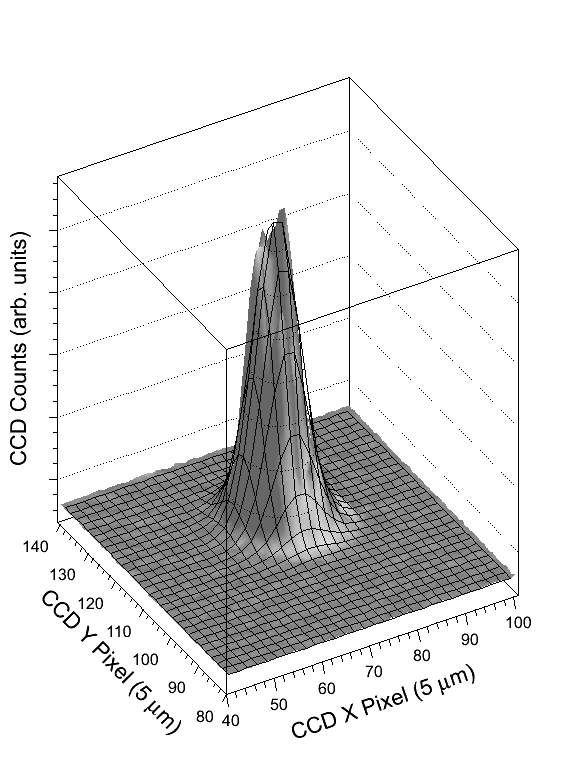
\includegraphics[width=.33\textwidth]{figures/astig_thesis_2Dgaus_run35.png}
                ~
                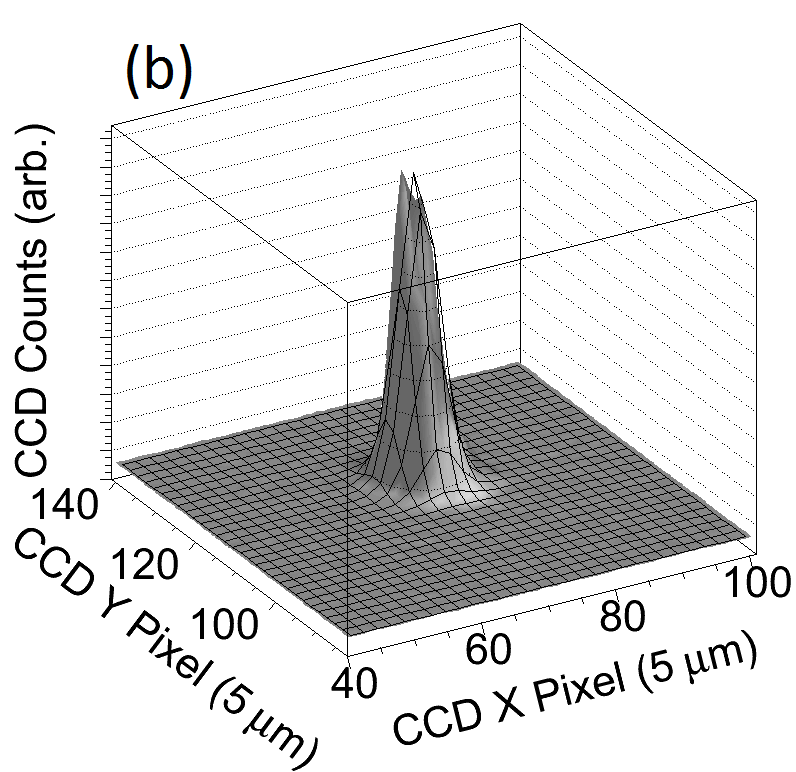
\includegraphics[width=.33\textwidth]{figures/astig_thesis_2Dgaus_run39.png}
                ~
                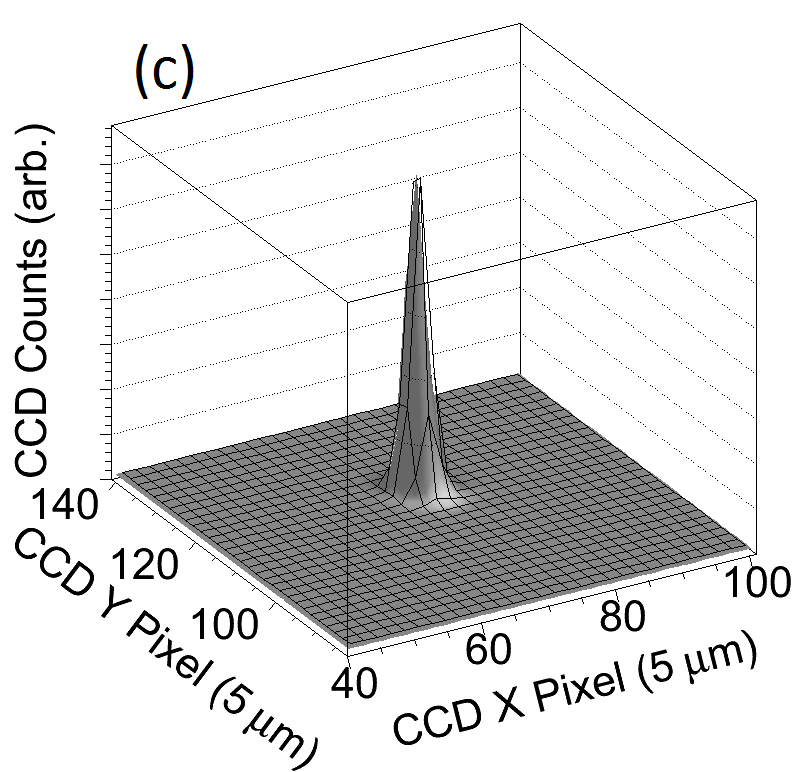
\includegraphics[width=.33\textwidth]{figures/astig_thesis_2Dgaus_run43.png}
                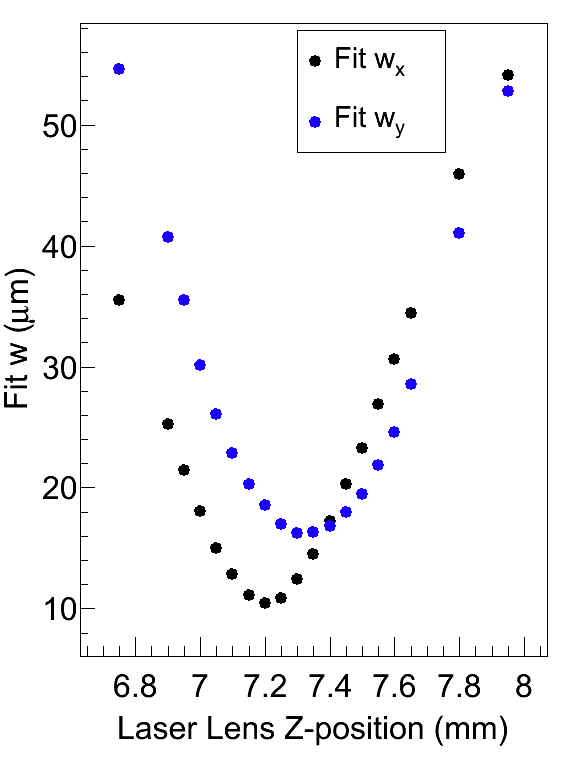
\includegraphics[width=.45\textwidth]{figures/astigcorr_curve_no-corr_806.png}
                ~
                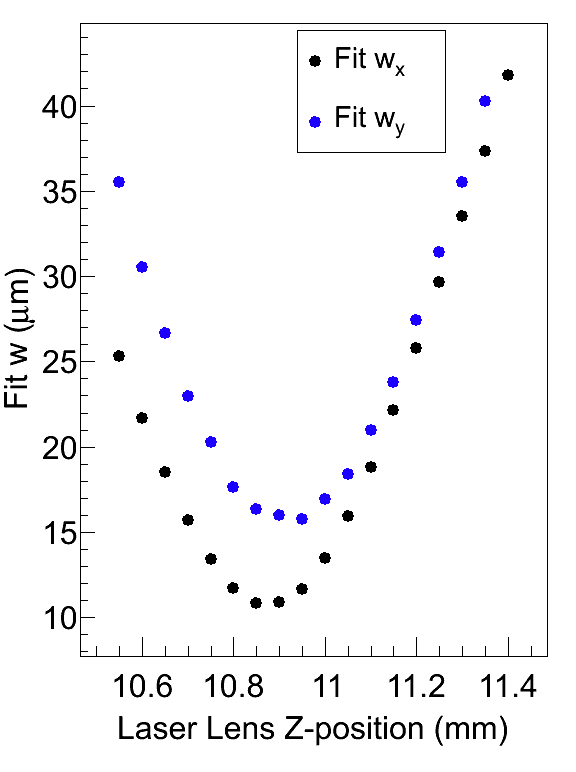
\includegraphics[width=.45\textwidth]{figures/astigcorr_curve_corr_10deg.png}
                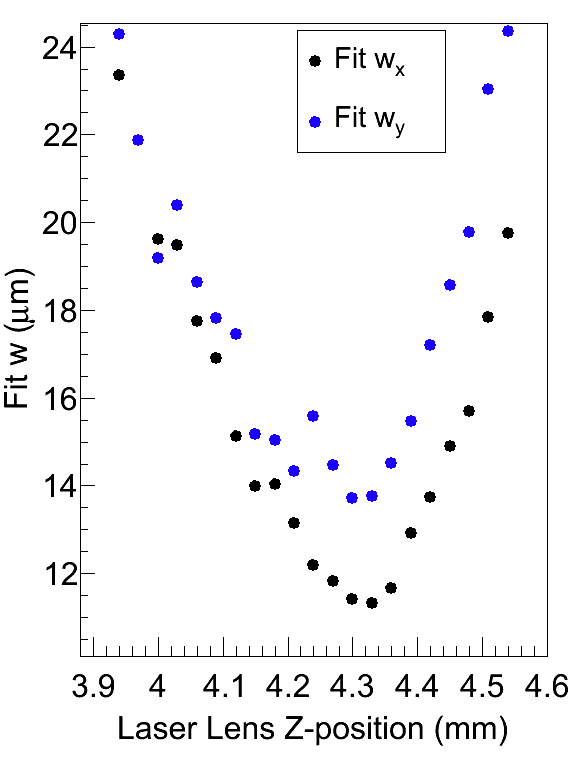
\includegraphics[width=.45\textwidth]{figures/astigcorr_curve_corr_9-16.png}
                ~
                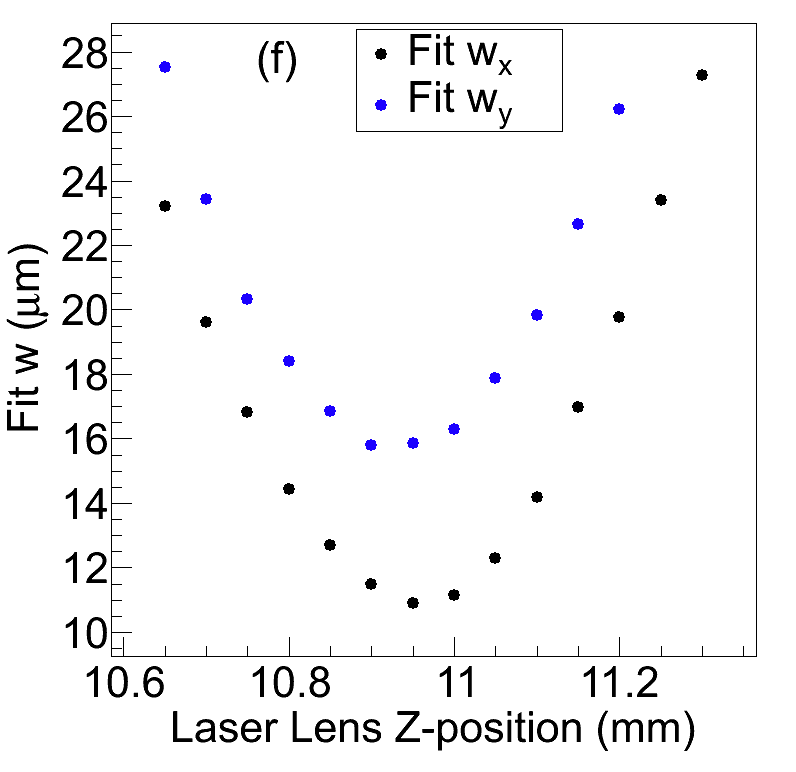
\includegraphics[width=.45\textwidth]{figures/astigcorr_curve_corr_13deg.png}
                \caption{Example 2D Gaussian fits (black grid lines) with varying laser z position (a,b,c), and fit radii  w$_{\text{x}}$ (black) and  w$_{\text{y}}$ (blue) vs. laser focus lens position with (d) no compensator, and with compensator at about (e) 10$^{\circ}$, (f) 11$^{\circ}$, and (g) 13$^{\circ}$.}
\label{fig:astig}
\end{figure}	

The tilted sapphire window introduces astigmatism to the focused laser.  To correct for this, compensating astigmatism is introduced by a fused silica optical flat of 1~cm thickness, placed after the lens, tilted in the y plane (the laser is along the z-direction, and the sapphire window is tilted in the x plane).  The proper angle for the compensator was determined to be about 10$^{\circ}$ from normal by a ray matrix calculation \cite{raymatrix}.  The astigmatism of the SXe layer is negligible since its thickness is only about half a micron in a typical fluorescence experiment.  With the compensator, overlapping minimum spot sizes of 2.06~$\mu$m and 2.66~$\mu$m are calculated for x and y, respectively.

To observe the astigmatism and the effect of the compensator, the relative positions in z of the x and y foci were observed by imaging 619-nm Ba fluorescence from a large deposit of Ba\textsuperscript{+} in SXe, with a varying laser focus.  For each z-position of the laser focusing lens, an image was taken, and a 2D Gaussian fit determined the 1/$e^{2}$ x- and y- radii, w$_{\text{x}}$ and w$_{\text{y}}$, of the image.  Although these radii are significantly larger than that of the laser beam due to SXe surface scattering and collection optics imperfections, the z-position of the best focus can be accurately determined.  Example fits to the 619-nm fluorescence images for three laser focus positions, using the astigmatism compensator at 10$\pm 1^{\circ}$, are shown in Fig. \ref{fig:astig}(a,b,c).  Gaussian fit values for w$_{\text{x}}$ and w$_{\text{y}}$ are plotted vs. laser focus position with (d) no compensator, and with the compensator at (e) 10$\pm 1^{\circ}$, (f) 11$\pm 1^{\circ}$, and (g) 13$\pm 1^{\circ}$.  With no compensator (d), the focal positions for x and y are measured to be 127.6$ \pm 2.5$~$\mu$m apart.  Compensation angles 10$\pm 1^{\circ}$ (e) and 13$\pm 1^{\circ}$ (g) can be seen to under- and over-shoot the optimal angle, respectively.  The angle 11$\pm 1^{\circ}$ (f), which was used in imaging experiments, is near optimal, i.e. the x and y focal positions are consistent to within 45~$\mu$m.  %\emph{\color{gray}A systematic uncertainty... on the beam size is then obtained ... leading to a focused laser spot of ?? $\pm$ ?? $\mu$m\textsuperscript{2} [get this uncertainty from error propagation of angle(s) through gaussian beam ray matrix}

The laser spot size ($A_{\text{laser}}$) is defined as the area enclosed within the 1/$e$ radii of the laser beam, according to Eq. \ref{eqn:laserspot}:

\begin{equation}
A_{\text{laser}} = \frac{\pi w_{x} w_{y}}{2}
\label{eqn:laserspot}
\end{equation}

\noindent
where $w_{x,y}$ are the $x$ and $y$ 1/$e^{2}$ radii of the focused laser in the SXe.  In the case of the bi-convex lens, $w_{x} \approx w_{y} \equiv w$.

%\emph{\color{gray}which is consistent with the calculated value of {\color{red}??}~$\mu$m from...}

%[waist measurements? -- apply calibration uncertainty to the good motor-stage ones]

%show measurements of astig. w/ and w/o compensator.?  8-7 prolly best so far

%Astigmatism in the laser itself was measured to be consistent with zero. (pg. 24 of Chris's book)
\section{Collection Optics}
\label{sec:collection}

Fluorescence is collected above the cryostat, as shown in Fig. \ref{fig:endOfBeamOptics}.  A 50~mm Nikon camera lens collimates the light, and one or more fluorescence filters sit on top of it.  A band-pass filter is used for imaging, and a Raman filter is used for spectroscopy.  The fluorescence is then guided by two steering mirrors, and is imaged by a 200~mm Nikon camera lens onto a Roper Scientific liquid-nitrogen-cooled CCD, with a net magnification of 4.  The CCD has a quantum efficiency of 90\% in the visible, and in its medium gain mode, records one count per four photoelectrons collected.  At the set point of -100~$^{\circ}$C, dark counts are negligible.

For spectroscopy, the 200~mm camera lens focuses the light onto the inlet slit of an Acton SP-2150i imaging spectrometer, which is then imaged by the spectrometer onto the CCD after reflecting off a diffraction grating.  The 0-order reflection of the grating provides an image for alignment, and the grating can be tilted to distribute the 1\textsuperscript{st}-order reflection across the horizontal CCD pixels for doing spectroscopy.

When a 1" diameter filter is used, the imaging system has a solid angle collection of about 1.5\%.  Each additional component in the collection optics, listed in Table \ref{table:colleff}, contributes some loss, resulting in a total collection efficiency ($\epsilon_{c}$) of $1.1 \times 10^{-3}$ with the spectrometer, and $2.1 \times 10^{-3}$ without.  The spectrometer also limits the system to an f-number of 4, though this is not limiting in this setup.

\begin{table} [!htbp]
\caption{Factors contributing to optical collection efficiency.  Total $\epsilon_{c}$ includes 1.5\% solid angle collection.}
\label{table:colleff}
\begin{tabular}{l l l}
Component & Efficiency & \\
\hline
Cryostat Window & 0.99 & \\
Camera Lens 50~mm & 0.89 & \\
Camera Lens 200~mm & 0.91 & \\
Steering Mirrors ($\times 2$) & 0.95 & \\
CCD Quantum Efficiency & 0.90 & \\
Filter & 0.98 & \\
Counts per Photoelectron (CCD) & 0.22 & $\epsilon_{c}\text{(w/o spectrom.)} = 2.1 \times 10^{-3}$\\
\hline
Spectrometer & 0.5 & $\epsilon_{c}\text{(w/ spectrom.)} = 1.1 \times 10^{-3}$\\
\end{tabular}
\end{table}

%Spectrom. Mirrors ($\times 2$) & {\color{red}??} & \\
%Diffraction Grating & 0.5 & $\epsilon_{c}\text{(w/ spectrom.)} = ${\color{red}??}\\

To avoid unnecessary fluorescence bleaching, a laser shutter was linked to the camera shutter with a LabVIEW program.  This program also recorded laser power via a calibrated pickoff, as well as the temperature of the coldfinger near the sapphire window during observation.

%the laser exposure was limited to only the time of CCD exposure using

Although the imaging spectrometer can produce spacial images with the 0-order grating reflection, better collection efficiency and imaging quality are achieved by removing the spectrometer and imaging directly onto the CCD.  Band-pass filters were used to pass the desired Ba fluorescence peak(s) while greatly attenuating laser scatter and sapphire fluorescence.

%angle=90,
\begin{figure} %[H]
        \centering
                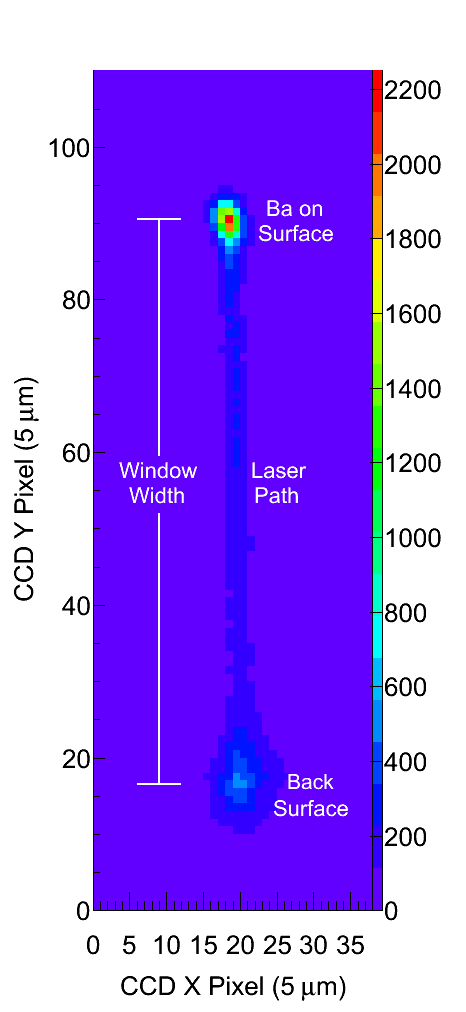
\includegraphics[width=.4\textwidth]{figures/imageExamp.png}
                \caption{Example image of focused laser exciting a Ba\textsuperscript{+} deposit on a c-plane sapphire window of 0.5~mm thickness.  Fluorescence is passed by 620-nm band-pass filter.}
\label{fig:imageexamp}
\end{figure}

An example raw image of the focused 570~nm dye laser on a Ba\textsuperscript{+} deposit using the fluorescence of the 619-nm peak is shown in Fig. \ref{fig:imageexamp}.  With 4$\times$ magnification, each pixel corresponds to 5~$\mu$m$\times$5~$\mu$m on the window.  The laser's path through the window is faintly visible by the residual broad Cr\textsuperscript{3+} fluorescence that is passed by the 620-nm band-pass filter.  The laser is focused at the top surface of the window, which faces the ion beam.  The surface background is seen on the back surface, and the 619-nm Ba fluorescence stands out above both backgrounds on the top surface.  The imaging resolution results in a 1/e$^{2}$ radius of about 12~$\mu$m when imaging the 2.06~$\mu$m $\times$ 2.66~$\mu$m 1/e$^{2}$ laser spot.

\section{Wavelength Calibration}

Wavelength calibration of the spectrometer was done using three lasers whose wavelengths were first measured with a Burleigh Wavemeter:  a red diode laser at 656.99~nm, a doubled Nd:YAG laser at 532.23~nm, and the C480 blue dye laser typically around 475~nm.  These lasers were directed at the same position on the sapphire window, and their scatter was imaged along the same path as the Ba fluorescence.  The WinSpec software applies the diffraction grating equation to calibrate each CCD pixel to a wavelength.

\section{Vibrations and Effective Laser Region}
\label{sec:vibes}

\begin{figure} %[H]
        \centering
                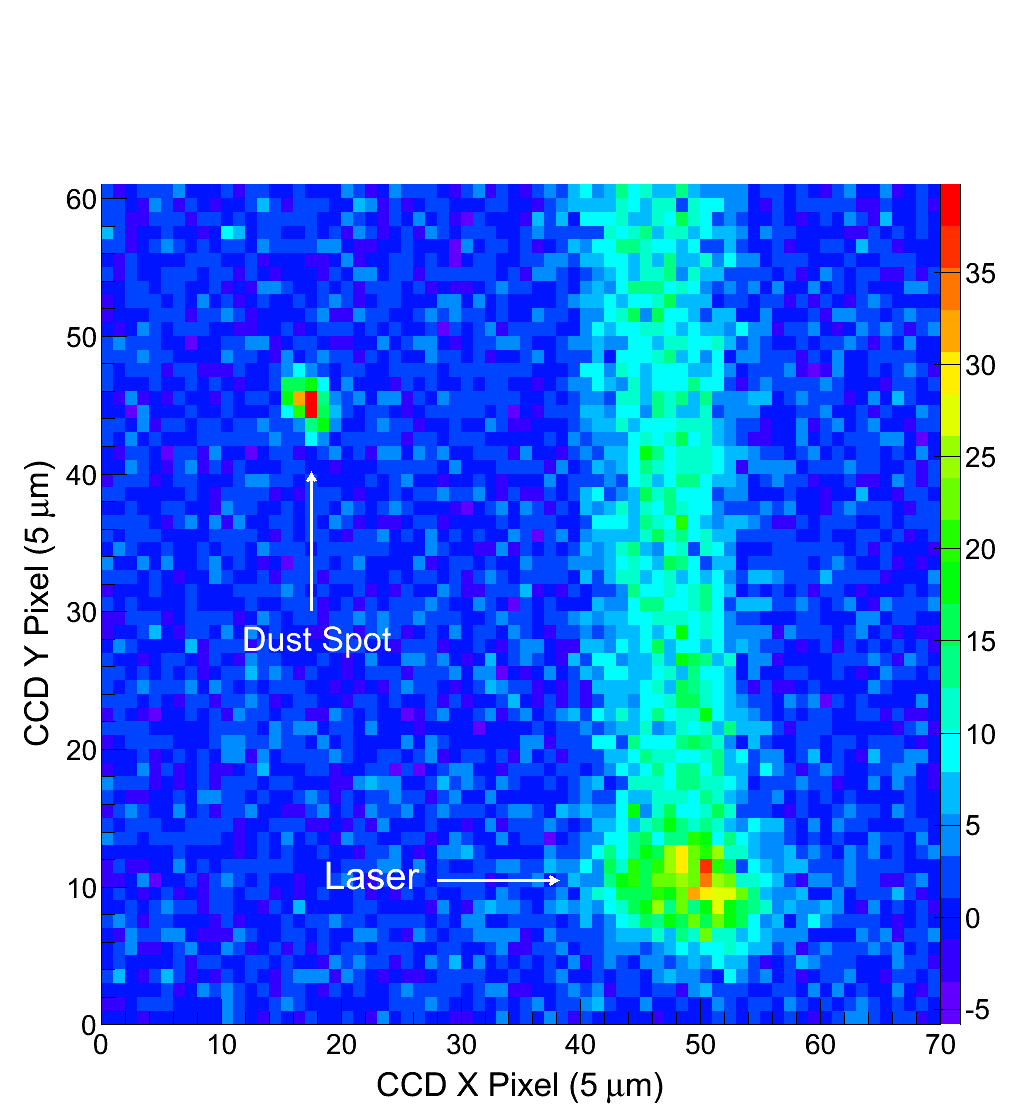
\includegraphics[width=.6\textwidth]{figures/image_dustspot.png}
                \caption{Example image of dust spot and laser during observation of cryostat vibrations.}
\label{fig:dustspot}
\end{figure}

\begin{figure} %[H]
        \centering
                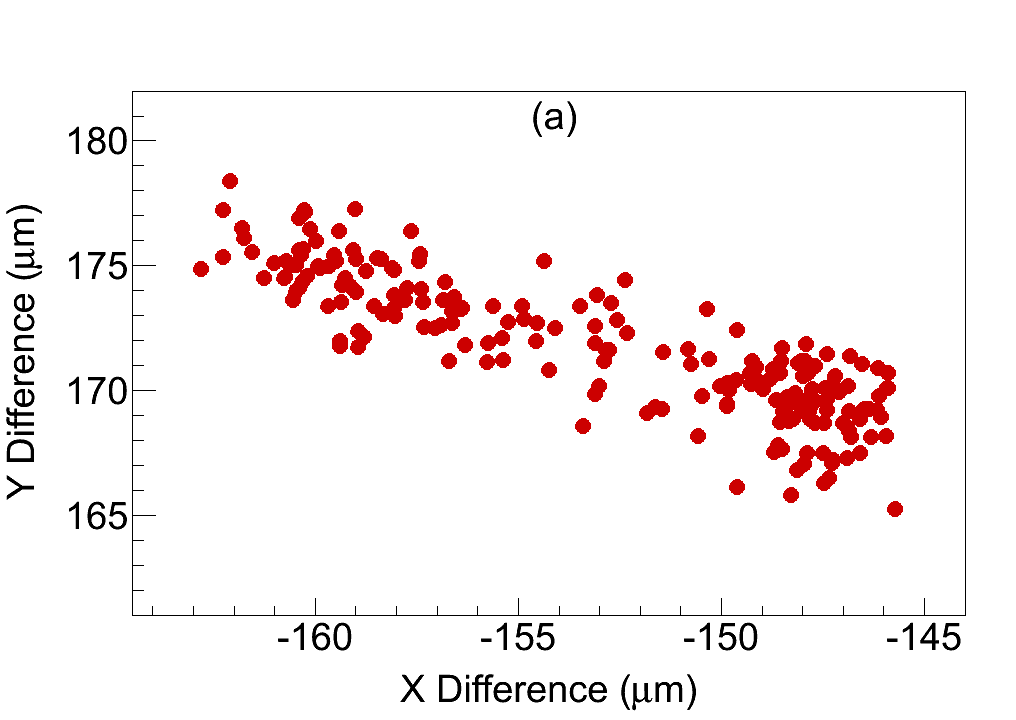
\includegraphics[width=.5\textwidth]{figures/cryovibes_a.png}
                ~
                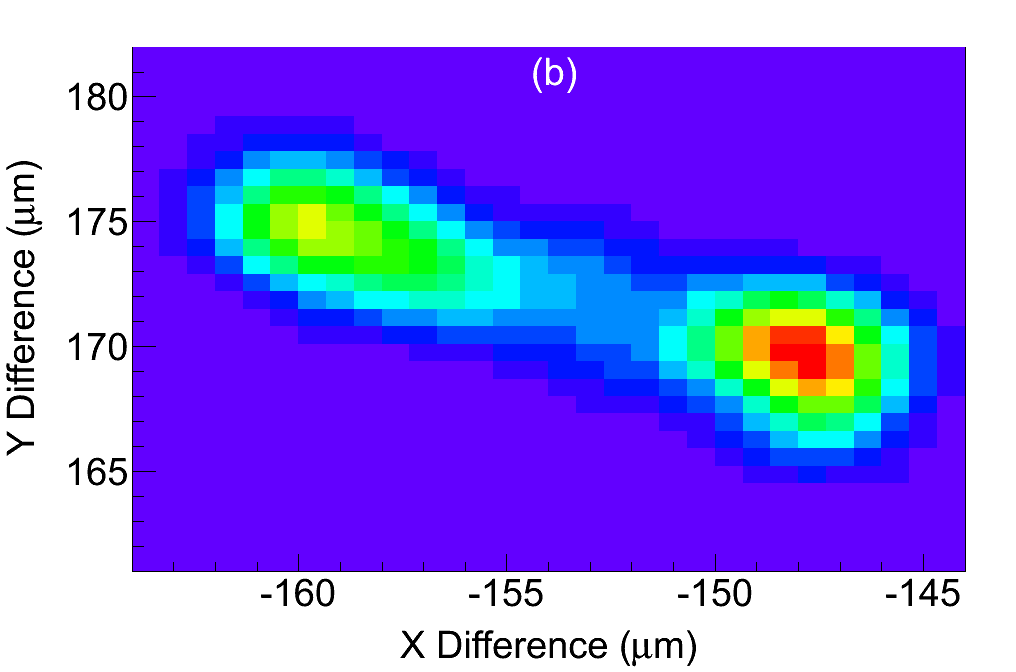
\includegraphics[width=.5\textwidth]{figures/cryovibes_b.png}
                \caption{Cryostat vibration measurements based on relative position of dust spot vs. laser on sapphire window in 50-ms snapshots (a), with 2D Gaussians of w$_{\text{x}} \times $w$_{\text{y}}$ = $2.06~\mu$m$ \times 2.66~\mu$m overlain on each point to represent total laser exposure vs. position (b).}
\label{fig:cryovibe2D}
\end{figure}

Relative vibrations between the laser and the sapphire window occur from a few sources.  Firstly, the laser is on a separate optical table from the cryostat and collection optics.  Secondly, the cryostat has some vibration due to its He pump cycles.  Vibrations affect the total number of Ba atoms exposed during a measurement, but not the instantaneous number of Ba atoms in the laser beam area.  Vibrations were observed by determining the position of a ``dust spot" (a highly scattering feature on one sapphire window) relative to the position of the laser in an image on time scales down to 50~ms.  An example of an image from this experiment is shown in Fig. \ref{fig:dustspot}.  The dust spot was illuminated by a de-focused 657~nm diode laser, and the 570-nm dye laser was somewhat de-focused in order to optimally de-focus the red laser with the same focusing lens. For each frame, 2D Gaussian functions with variable widths and magnitudes were fit to locate the center of the laser spot and the dust spot in order to measure their relative position.  The fit range for the laser spot was restricted in y so that it was not affected by the bulk sapphire fluorescence path.  The distances in x and y between the dust spot and laser are plotted for each 50-ms snapshot in Fig. \ref{fig:cryovibe2D}(a).  The distribution shows a correlation between x and y, indicating vibration in a particular direction.  The amplitude of the vibration is about 15~$\mu$m from this data.  To calculate an effective laser spot size due to this vibration, each difference (x,y) between laser and dust spot was used as the center of a 2D Gaussian, each with w$_{x} = 2.06~\mu$m and w$_{y} = 2.66~\mu$m to represent the laser spot.  Such Gaussian functions were summed for all points to produce a distribution of summed laser exposure, shown in Fig. \ref{fig:cryovibe2D}(b).  The area enclosed by a 1/e contour then is a measure of the effective total exposed area.  On the other hand, signal at a given moment is still emitted only from the laser spot size.  Then there are two possible definitions for the number of ions in the laser region, and thus the upper limit on the number of atoms.  In the absence of signal bleaching, the instantaneous number of atoms exposed is a good definition for the number of atoms observed.  If there is large bleaching, the more conservative estimate is more appropriate.  Note that the factor between instantaneous and total exposure areas depends on the laser spot size.  The factor is about 4.7 for w$_{\text{x}} \times $w$_{\text{y}}$ = $2.06~\mu$m$ \times 2.66~\mu$m (astigmatism compensation and no spherical aberration), and about 3 for w$_{\text{x}} \times $w$_{\text{y}}$ = $5~\mu$m$ \times 5~\mu$m.

%In the absence of signal bleaching, the average number of atoms exposed is a good definition for the number of atoms observed.

%Since x and y movement are correlated, and since the movement is sinusoidal, the effective area is only about 5$\times$ the real laser spot size, and the effective laser region is about 40~$\mu$m$^{2}$.

%The difference between dust spot and laser positions is plotted in {\color{red}Fig. [fig vibe vs. time with sine fit]} for both x and y.  Each exposure in this plot is 50~ms, though readout time and camera shutter compensation time result in x~s between frames.  The best fit of a sine function results in a vibration frequency of x~Hz.  This is consistent with the audible frequency of the cryostat He pump.
%...could do this for rotated

For imaging of single Ba atoms, the relative vibration is the vibration of most concern.  Vibration of the laser itself is seen to be small in this study.  Vibration of the collection optics will affect the imaging resolution, but not the number of atoms being observed, or the resolution of a single atom iamge in a laser raster scan.  These vibrations were minimized by stable mounting on large diameter posts.

%\vspace{10mm}

\begin{figure} %[H]
        \centering
                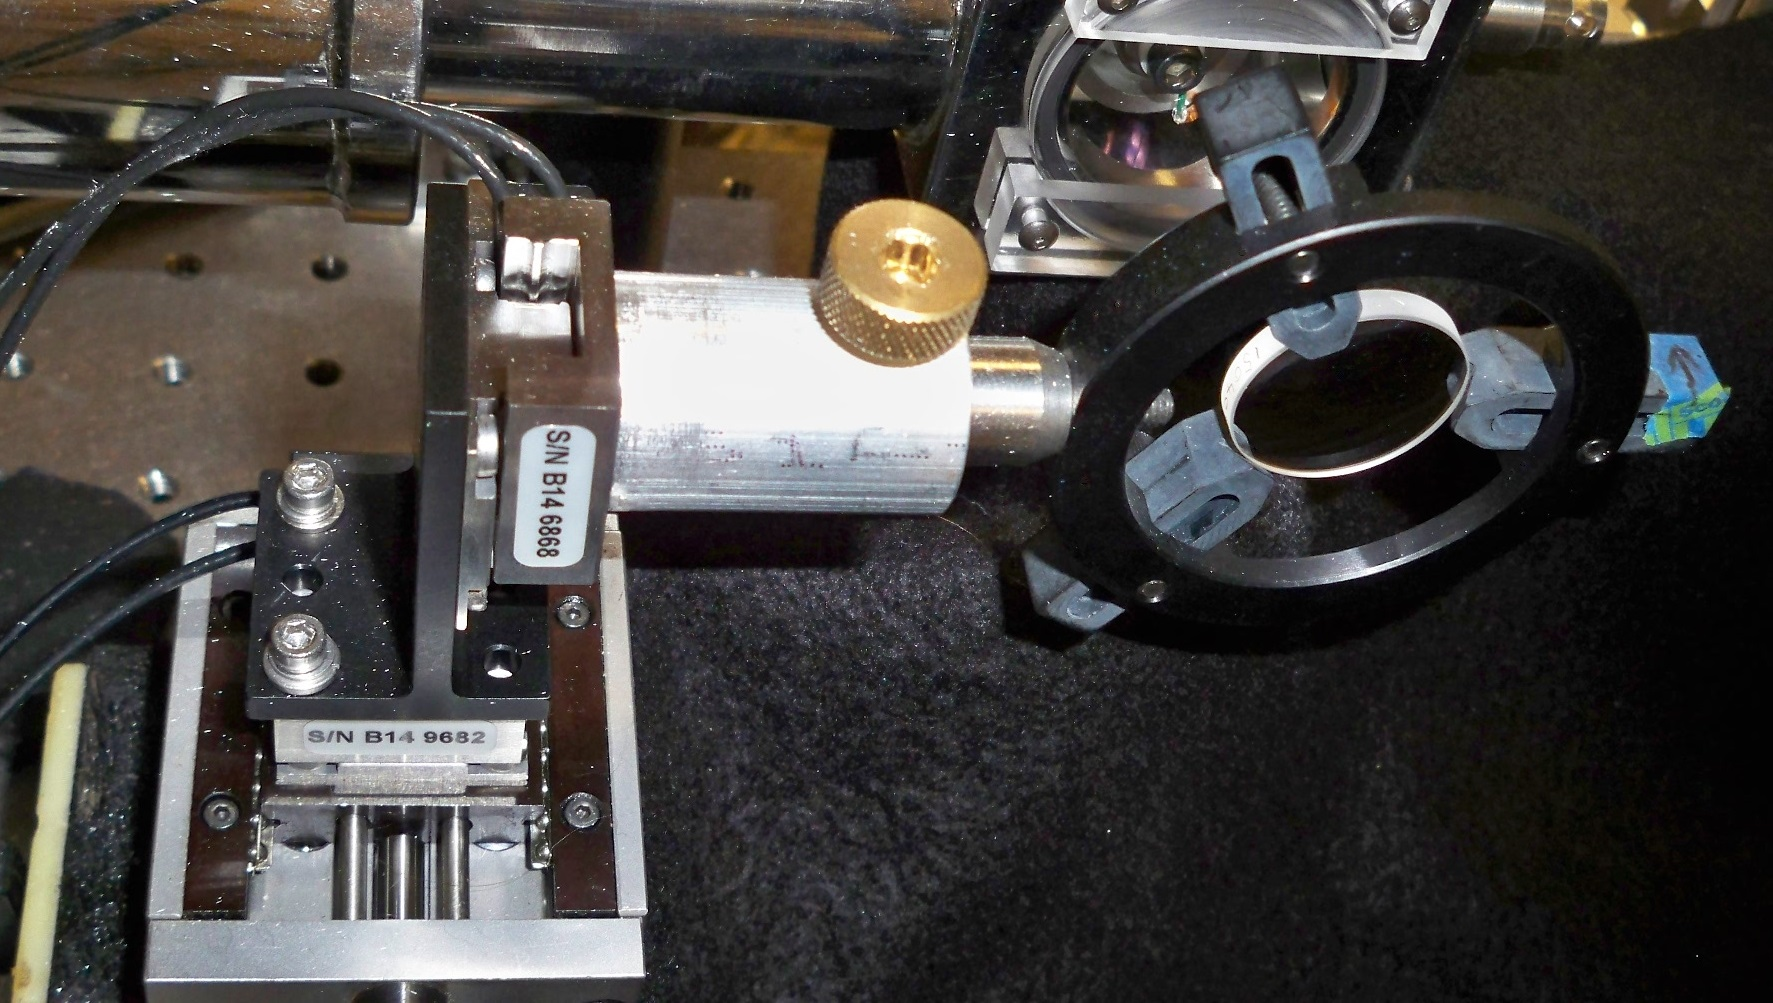
\includegraphics[width=.5\textwidth]{figures/stages_2.JPG}
                \caption{Asphere laser focusing lens mounted to two motorized Newport translation stages for laser scanning in x and y.}
\label{fig:laserStages}
\end{figure}


\section{Laser Scanning}
\label{sec:laserscanning}

In order to obtain images of separated single atoms, the laser focusing lens is attached to motorized translation stages which scan the laser position by scanning the lens in x and y, as shown in Fig. \ref{fig:laserStages}.  These stages sat atop a manual z-translation stage for laser focusing.  A LabVIEW program coordinates movement of these stages such that x or y position is stepped in between CCD frames, and each frame then corresponded to a position in a laser scan grid.

Relative laser-window vibration may be eliminated by using a different cryostat, or by gating the laser with a shutter to block exposure during He pump surges.  With no vibration, resolution of Ba atoms in scanned images is limited only by the size of the laser beam, not by the resolution of the collection optics and the CCD pixel size.

%\emph{\color{red}The stages used in this work were Newport AG-LS25, which are driven by piezoelectric motors, but without accurate position feedback.  As a result, some inconsistency in position reproducibility was observed.  The position of the focused laser, measured by the center of a 2D Gaussian fit to the image of the laser spot, is shown in Fig. [fig laser grid] for ... 2015-08-12 has one from chris where he did 2D gaus, but you should get that w/ them lined up from the start too, to separate init pos from inconsistency, and you need to quantify both}

%\emph{\color{gray}Show data on steps and reproducibility -- say this isn;t good and new stages will be used later.}